% Font options: 10pm, 11pt, 12pt
% Align headings left instead of center: nocenter
\documentclass[xcolor=x11names,compress]{beamer}\usepackage[]{graphicx}\usepackage[]{color}
%% maxwidth is the original width if it is less than linewidth
%% otherwise use linewidth (to make sure the graphics do not exceed the margin)
\makeatletter
\def\maxwidth{ %
  \ifdim\Gin@nat@width>\linewidth
    \linewidth
  \else
    \Gin@nat@width
  \fi
}
\makeatother

\definecolor{fgcolor}{rgb}{0.345, 0.345, 0.345}
\newcommand{\hlnum}[1]{\textcolor[rgb]{0.686,0.059,0.569}{#1}}%
\newcommand{\hlstr}[1]{\textcolor[rgb]{0.192,0.494,0.8}{#1}}%
\newcommand{\hlcom}[1]{\textcolor[rgb]{0.678,0.584,0.686}{\textit{#1}}}%
\newcommand{\hlopt}[1]{\textcolor[rgb]{0,0,0}{#1}}%
\newcommand{\hlstd}[1]{\textcolor[rgb]{0.345,0.345,0.345}{#1}}%
\newcommand{\hlkwa}[1]{\textcolor[rgb]{0.161,0.373,0.58}{\textbf{#1}}}%
\newcommand{\hlkwb}[1]{\textcolor[rgb]{0.69,0.353,0.396}{#1}}%
\newcommand{\hlkwc}[1]{\textcolor[rgb]{0.333,0.667,0.333}{#1}}%
\newcommand{\hlkwd}[1]{\textcolor[rgb]{0.737,0.353,0.396}{\textbf{#1}}}%
\let\hlipl\hlkwb

\usepackage{framed}
\makeatletter
\newenvironment{kframe}{%
 \def\at@end@of@kframe{}%
 \ifinner\ifhmode%
  \def\at@end@of@kframe{\end{minipage}}%
  \begin{minipage}{\columnwidth}%
 \fi\fi%
 \def\FrameCommand##1{\hskip\@totalleftmargin \hskip-\fboxsep
 \colorbox{shadecolor}{##1}\hskip-\fboxsep
     % There is no \\@totalrightmargin, so:
     \hskip-\linewidth \hskip-\@totalleftmargin \hskip\columnwidth}%
 \MakeFramed {\advance\hsize-\width
   \@totalleftmargin\z@ \linewidth\hsize
   \@setminipage}}%
 {\par\unskip\endMakeFramed%
 \at@end@of@kframe}
\makeatother

\definecolor{shadecolor}{rgb}{.97, .97, .97}
\definecolor{messagecolor}{rgb}{0, 0, 0}
\definecolor{warningcolor}{rgb}{1, 0, 1}
\definecolor{errorcolor}{rgb}{1, 0, 0}
\newenvironment{knitrout}{}{} % an empty environment to be redefined in TeX

\usepackage{alltt}
%\documentclass[xcolor=x11names,compress,handout]{beamer}
\usepackage[]{graphicx}
\usepackage[]{color}
\usepackage{booktabs}
\usepackage{hyperref}
\usepackage{tikz}
\usepackage{multirow}
\usepackage{dcolumn}
\usepackage{bigstrut}
\usepackage{amsmath} 
\usepackage{xcolor,colortbl}
\usepackage{amssymb}
%\newcommand{\done}{\cellcolor{teal}#1}

%% Beamer Layout %%%%%%%%%%%%%%%%%%%%%%%%%%%%%%%%%%
\useoutertheme[subsection=false,shadow]{miniframes}
\useinnertheme{default}
\usefonttheme{serif}
\usepackage{Arev}
\usepackage{pdfpages}

\setbeamerfont{title like}{shape=\scshape}
\setbeamerfont{frametitle}{shape=\scshape, size=\normalsize}

\definecolor{dkblue}{RGB}{0,0,102}

\setbeamercolor*{lower separation line head}{bg=dkblue} 
\setbeamercolor*{normal text}{fg=black,bg=white} 
\setbeamercolor*{alerted text}{fg=red} 
\setbeamercolor*{example text}{fg=black} 
\setbeamercolor*{structure}{fg=black} 
 
\setbeamercolor*{palette tertiary}{fg=black,bg=black!10} 
\setbeamercolor*{palette quaternary}{fg=black,bg=black!10} 

\renewcommand{\(}{\begin{columns}}
\renewcommand{\)}{\end{columns}}
\newcommand{\<}[1]{\begin{column}{#1}}
\renewcommand{\>}{\end{column}}

\setbeamertemplate{navigation symbols}{} 
\setbeamertemplate{footline}[frame number]
\setbeamertemplate{caption}{\raggedright\insertcaption\par}

\setbeamersize{text margin left=5pt,text margin right=5pt}

%%%%%%%%%%%%%%%%%%%%%%%%%%%%%%%%%%%%%%%%%%%%%%%%%%


\title{Making Causal Critiques}
\subtitle{Day 4 - How much are we Learning?}
\author{Jonathan Phillips}
\IfFileExists{upquote.sty}{\usepackage{upquote}}{}
\begin{document}

\frame{\titlepage}

\section{Introduction}

\begin{frame}
\frametitle{How much are we Learning?}
\begin{itemize}
\item Everything we have discussed so far has been about the \textbf{accuracy} of a causal claim
\item But not every study is as valuable to political science
\item We \textit{learn} more from some studies than from others
\begin{enumerate}
\item Reliability of the claim
\item Reproducibility of the claim
\item Scope (\textit{generalizability}) of the claim
\end{enumerate}
\end{itemize}
\end{frame}

\begin{frame}
\frametitle{Robustness}
\begin{itemize}
\item For simplicity, we publish a paper with a 'final' result
\begin{itemize}
\item 1\% extra GDP growth increases the President's chance of re-election by 5\%
\item One more year of drought increases the risk of conflict by 10\%
\end{itemize}
\item But how \textbf{confident} are we in these figures?
\item Good studies include estimates of uncertainty
\begin{itemize}
\item 1\% extra GDP growth increases the President's chance of re-election by 5\% with a standard deviation of 0.2\%
\item One more year of drought increases the risk of conflict by 10\%, with a standard deviation of 30\%
\end{itemize}
\item But these confidence intervals are usually for a \textit{single} methodology and set of assumptions
\end{itemize}
\end{frame}

\begin{frame}
\frametitle{Robustness}
\begin{itemize}
\item What if our assumptions were wrong?
\item How much would our results change if we used a different methodology?
\begin{itemize}
\item Including different controls
\item Including alternative measures of the variables
\item Including or excluding outliers
\end{itemize}
\item If we can change all these things and still get the same answers, our result is \textbf{reliable} and \textbf{robust}
\end{itemize}
\end{frame}

\begin{frame}
\frametitle{Robustness}
\begin{itemize}
\item For example, Michalpoulos and Papaioannou (2013) show that more centralized pre-colonial societies in Africa have more economic activity today
\item Robustness tests include:
\begin{itemize}
\item Extra controls for disease, land, natural resources
\item Alternative model for spatial autocorrelation
\item Country fixed effects to focus only on within-country variation
\item Comparing only neighbouring societies
\item Alternative codings of centralized pre-colonial societies
\item Alternative measures of economic activity (nightlights etc.)
\item Different units of analysis - grid squares instead of ethnic territories
\end{itemize}
\end{itemize}
\end{frame}

\begin{frame}
\frametitle{Robustness}
\begin{itemize}
\item Robustness tests help avoid \textbf{researcher bias}
\begin{itemize}
\item Running 200 models with different covariates
\item Only reporting one that is significant
\item But even if there was \textbf{no causal effect} in the data, \textit{by chance} we would expect 20 models to produce significant effects
\end{itemize}
\end{itemize}
\end{frame}

%altonji et al sensitivity analysis

\begin{frame}
\frametitle{Reproducibility}
\begin{enumerate}
\item If we take the same data and apply the same method, do we get the same result?
\begin{itemize}
\item Often, no! Only ~35\% in Brazilian political science journals (Avelino and Desposato 2018)
\end{itemize}
\item If we take another sample of data and apply the same method, do we get the same result?
\begin{itemize}
\item Very rarely done
\end{itemize}
\end{enumerate}
\end{frame}

\begin{frame}
\frametitle{Reproducibility}
\begin{itemize}
\item A big problem for reproducibility is \textbf{publication bias}
\begin{itemize}
\item Lots of researchers perform lots of studies
\item Some find positive results, some negative, many 'null' findings
\item But journals want readers, and readers like positive results
\item So only the positive results get published
\end{itemize}
\item If you're reading a paper, think of the ten other papers you're \textit{not} reading that tried the same thing and found no effect
\end{itemize}
\end{frame}

\begin{frame}
\frametitle{Reproducibility}
\begin{itemize}
\item One solution is \textbf{Pre-registration}
\begin{itemize}
\item Submit your study design to a website - what you will analyse and how
\item Everyone knows who is researching what, and if they published or not
\item Researchers are also less tempted to 'pick' their preferred analysis after seeing the data
\item Eg. \href{https://egap.org/content/registration}{EGAP Pre-Registration}
\end{itemize}
\end{itemize}
\end{frame}

\begin{frame}
\frametitle{Generalizability}
\begin{itemize}
\item But even if studies are robust and reproducible, \textbf{how much} are we learning?
\item We can learn very little even from a precise, bias-free study:
\begin{itemize}
\item \href{https://www.improbable.com/ig/winners}{IgNobel Prize}
\item "Suicide rates are linked to the amount of country music played on the radio"
\item "Is using voodoo dolls effective?"
\item "Why do old men have big ears?"
\item "How exposure to a crocodile encourages people to gamble"
\end{itemize}
\end{itemize}
\end{frame}

\begin{frame}
\frametitle{Generalizability}
\begin{itemize}
\item \textbf{Internal Validity}
\begin{itemize}
\item Are the conclusions of the study accurate \textit{within} the sample?
\item Are the assumptions valid, is our causal effect biased?
\item Is the conclusion reliable if we use slightly different assumptions?
\end{itemize}
\item \textbf{External Validity}
\begin{itemize}
\item How far can the results 'travel' outside of the study design?
\begin{enumerate}
\item Does the study reflect a wider population?
\item How big, representative and interesting is that wider population?
\end{enumerate}
\end{itemize}
\end{itemize}
\end{frame}

\begin{frame}
\frametitle{Generalizability}
\begin{itemize}
\item For example, Chattopadhyay and Duflo (2004) argue that women leaders invest more in education using data from 265 villages in two states in India (West Bengal and Rajasthan)
\item But does the conclusion hold if we get more data from:
\begin{enumerate}
\item 265 different villages?
\item Different states?
\item Different countries?
\item Different years?
\end{enumerate}
\end{itemize}
\end{frame}

\begin{frame}
\frametitle{Generalizability}
\begin{itemize}
\item Most studies are designed with generalizability in mind:
\begin{itemize}
\item Representative Samples are drawn from a target population
\item So we can use \textbf{statistical inference} to extend our conclusions from the sample to the population
\begin{itemize}
\item Note this only works if we know all the units (hidden tribes etc.)
\end{itemize}
\item But Chattopadhyay and Duflo (2004) did not take a representative sample of villages - they surveyed all villages in one district
\item Their widely-cited paper \textit{only} applies to Birbhum and Udaipur districts
\item We have no evidence of how women leaders govern elsewhere in India or the world
\end{itemize}
\end{itemize}
\end{frame}

\begin{frame}
\frametitle{Generalizability}
\begin{itemize}
\item Specific causal research designs also restrict the scope of our findings
\begin{itemize}
\item Precisely because we had to restrict our sample to find appropriate counterfactuals
\item The new comparisons are often less representative or interesting
\end{itemize}
\item \item Instead of an \textbf{Average Treamtent Effect (ATE)} they represent a \textbf{Local Average Treatment Effect (ATE)}
\begin{itemize}
\item A treatment effect applicable only to those people who were affected by the methodology's treatment: \textbf{compliers}
\end{itemize}
\end{itemize}
\end{frame}

\begin{frame}
\frametitle{Field Experiments}
\begin{itemize}
\item Field experiments require lots of compromises and assumptions
\begin{itemize}
\item Costs
\item Ethical restrictions
\item Consent
\end{itemize}
\item Implementation is limited to a small sample, often non-representative
\item And the findings \textit{only} apply to that sample
\item Or maybe only to a sub-group of that sample
\end{itemize}
\end{frame}

\begin{frame}
\frametitle{Field Experiments}
\begin{itemize}
\item External Validity Limitations of Field Experiments:
\pause
\begin{itemize}
\item What theory are we testing? Can't accumulate knowledge without theory. The causal mechanisms are still a black box.
\item Limited portability of findings - context matters for the treatment effects:
\begin{itemize}
\item Eg. CCTs improve child health only where clinics are available
\item Average effects may not apply to any individual
\end{itemize}s
\item Naive application of policy implications
\item How much do the results depend on researcher oversight?
\end{itemize}
\end{itemize}
\end{frame}

\begin{frame}
\frametitle{Lab Experiments}
\begin{itemize}
\item Problems generalizing from the lab:
\begin{itemize}
\item \textbf{Hawthorne effect}: Lab context influences behaviour, social desirability bias
\item \textbf{Context effects}: The real-world always provides more information, more history
\item \textbf{Process effects}: People care \textit{how} decisions are made
\item \textbf{Selection effects}: Actors in specific roles are rarely representative samples, 'WEIRD' or pro-social lab subjects
\end{itemize}
\end{itemize}
\end{frame}

\begin{frame}
\frametitle{Lab Experiments}
\begin{itemize}
\item The lab differs from the field:
\pause
\begin{itemize}
\item The stakes
\item The norms (specific norms of being an experimental subject)
\item The degree of scrutiny
\item The sample of individuals
\item The degree of anonymity
\end{itemize}
\end{itemize}
\end{frame}

\begin{frame}
\frametitle{Lab Experiments}
\begin{itemize}
\item Levitt and List 2006 argue lab experiments are \textit{inherently} flawed because the decisions we want to measure are likely to change depending on the degree of \textbf{scrutiny}
\pause
\item ``You tip more when you're on a date''
\item Social norms are activated, eg. treating one-shot games like repeated games
\item Scrutiny alters who wants to make a decision as well as the decision they make
\item Subjets use cues (heuristics) to draw on 'similar' situations from the real world
\end{itemize}
\end{frame}

\begin{frame}
\frametitle{Lab Experiments}
\begin{itemize}
\item Many studies find more cooperation in the lab than in the real world
\pause
\begin{itemize}
\item Scrutiny increases cooperation
\item Anonymity reduces cooperation
\item That's interesting in itself! We can manipulate the degree of scrutiny/anonymity etc.
\end{itemize}
\end{itemize}
\end{frame}

\begin{frame}
\frametitle{Lab Experiments}
\begin{itemize}
\item Lab experiments may be generalizable where norms/morality are less important
\pause
\begin{itemize}
\item ???
\end{itemize}
\end{itemize}
\end{frame}

\begin{frame}
\frametitle{Survey Experiments}
\begin{itemize}
\item Treatment occurs \textit{within} the survey questionnaire
\begin{itemize}
\item Different versions of the questionnaire randomly applied
\item Not a field experiment: Still an artificial context
\item Not a lab experiment: People not brought to a single location or interacting
\end{itemize}
\end{itemize}
\end{frame}

\begin{frame}
\frametitle{Conjoint Survey Experiments}
\begin{itemize}
\item How do people make choices between many options?
\item Treatments are often 'bundles', but which aspect matters most?
\end{itemize}
\end{frame}

\begin{frame}
\frametitle{Conjoint Survey Experiments}
\begin{itemize}
\item Hainmueller et al 2013 - How do attitudes to immigrants depend on immigrant characteristics?
\pause
\item Vary education, profession, language, gender, national origin, etc.
\item Profiles
\begin{itemize}
\item Attributes
\begin{itemize}
\item Values
\end{itemize}
\end{itemize}
\item Randomize attribute order to prevent bias
\end{itemize}
\end{frame}

\setbeamercolor{background canvas}{bg=}
\includepdf[pages={6}]{Jens.pdf}

\setbeamercolor{background canvas}{bg=}
\includepdf[pages={21}]{Jens.pdf}

\begin{frame}
\frametitle{Conjoint Survey Experiments}
\begin{itemize}
\item How realistic are the responses?
\begin{itemize}
\item Not a behavioural measure; nothing at stake
\item Social desirability bias
\item Not like real-world preference-formation process
\end{itemize}
\item Hainmueller et al 2014 - compare conjoint responses to a Swiss referendum
\item Citizens voted on specific naturalization applicants (Really!)
\end{itemize}
\end{frame}

\setbeamercolor{background canvas}{bg=}
\includepdf[pages={22}, scale=1.6, offset=0 -2.5cm]{Hainmueller2014.pdf}

\begin{frame}
\frametitle{Conjoint Survey Experiments}
\begin{itemize}
\item But note the conjoint method still hugely under-estimated the overall rejection rate
\item 21\% versus 37\% in reality
\end{itemize}
\end{frame}

\begin{frame}
\frametitle{Regression Discontinuity}
\begin{itemize}
\item The LATE is for those people who were so close to the discontinuity that whether they were treated or not is basically random
\begin{itemize}
\item Even though those cases are rare (eg. tied elections)
\item Even though we use data from a lot more people to estimate the LATE
\end{itemize}
\item Do we care about those people at the discontinuity?
\end{itemize}
\end{frame}

\begin{frame}
\frametitle{Regression Discontinuity}
\begin{itemize}
\item For example, Titiunik et al (2011) use a regression discontinuity on close elections in Brazilian municipalities to show that incumbent Mayors are more likely to lose (negative incumbency effect)
\begin{itemize}
\item But this does \textbf{not} mean that there is a negative incumbency effect in most Brazilian municipalities
\item Only about 500 out of 5,570 municipalities had 'close' elections (within +/-3\%)
\item Those municipalities were more urban, southern and wealthy than the rest
\item We do not learn anything about places where the result was a landslide (70-80\%)
\begin{itemize}
\item But these are the places where incumbents probably benefitted a lot!
\end{itemize}
\end{itemize}
\end{itemize}
\end{frame}

\begin{frame}
\frametitle{Regression Discontinuity}
\begin{itemize}
\item Similarly, geographic regression discontinuities only tells us the effect of living on one side of the border \textit{for people who live by the border}
\begin{itemize}
\item But who chooses to live by a border? People who like rural areas, migrants etc.
\item Self-selection bias has come back!
\end{itemize}
\end{itemize}
\end{frame}

\begin{frame}
\frametitle{Instrumental Variables}
\begin{itemize}
\item Critique (Deaton 2009):
\pause
\begin{itemize}
\item Our causal models need to represent a theory, not just be an arbitrary equation
\pause
\item If we use 'convenient' instruments, our causal effect and complier population are out of our control and might not be interesting
\pause
\item LATE causal estimates are not a good guide to policy effects
\pause
\item 'External' to our model is not the same as 'Exogenous', and we can't test exogeneity
\pause
\item Where the instrument is an arbitrary rule, there is often sorting as people re-adjust
\end{itemize}
\end{itemize}
\end{frame}

\begin{frame}
\frametitle{Learning in Political Science}
\begin{itemize}
\item So how much can we learn?
\begin{itemize}
\item We have to make careful judgments based on internal and external validity
\item Ideally combining multiple methodologies to compare low-bias low-generalizibility evidence with high-bias high-generalizability evidence
\end{itemize}
\end{itemize}
\end{frame}





\end{document}
 
 % effects of causes vs. reverse
